\documentclass[12pt,a4paper]{article}
\usepackage[utf8]{inputenc}
\usepackage{amsmath}
\usepackage{amsfonts}
\usepackage{amssymb}
\usepackage{graphicx}
\usepackage[left=1.00in, right=1.00in, top=1.00in, bottom=1.00in]{geometry}
\usepackage{fontspec}
\setmainfont{Times New Roman}

\usepackage{enumerate}
\usepackage{booktabs}
\usepackage{fontspec}
\usepackage{bm}
%minted --insert code
%\usepackage{minted}
%\usepackage{xcolor}
%\definecolor{background-color}{HTML}{f3f3f3} %background-color
%\newcommand{\inputmintedfile}[2]{
%	\inputminted[linenos=true,
%	bgcolor=background-color,
%	fontsize= \footnotesize,
%	fontfamily=courier ,
%	breaklines=true
%	]{#1}
%	{#2}
%}
%algorithm redefine
\usepackage{algorithm}
\usepackage{algorithmicx}
\usepackage{algpseudocode}
\renewcommand{\algorithmicrequire}{\textbf{Input:}}
\renewcommand{\algorithmicensure}{\textbf{Output:}}
\renewcommand{\thesection}{\arabic{section}.} 
\renewcommand{\thesubsection}{\roman{subsection}.}


\author{Zuyao Chen  201728008629002\\
	zychen.uestc@gmail.com}
\title{Assignment 4 of Algorithm}
\date{} 



\begin{document}
	\maketitle
\section{Integer Programming}

\textbf{Proof:} \\
\begin{itemize}
	\item Certificate: we can verify the constraints $Ax \geq b $ in polynomial time, thus it is a NP problem;
	\item NP-hard: Now we show that $\text{3-SAT} \leq_{P} \text{Integer Programming}$.
	Let $C_i$($i=1,2,...,m$) be the clauses of 3-SAT problem $\phi = C_1 \wedge C_2 \wedge \cdots \wedge C_m$, $x = (x_1,x_2,...,x_n)$.Once we construct a matrix $A$ and $b$ that each clause $C_i$ can be True or False corresponding to the True or False of the constraint $ a_{i1}x_1 + a_{i2}x_2 + ... + a_{in}x_n \geq b_i$
	, then $\phi$ is satisfied iff $Ax \geq b$ holds. \\
	For instance, $m=3$, $n =4$, $x_i = \{0,1\}$, $\phi =  (x_1 \vee x_2 \vee \neg x_3) \wedge (\neg x_1 \vee x_2 \vee x_4   ) \wedge (x_2 \vee x_3 \vee   x_4)$.  The corresponding constraints are $x_1 + x_2 + (1-x_3) \geq 1$,	$(1-x_1) + x_2 + x_4 \geq 1$ and 
	$ x_2 + x_3 + x_4 \geq 1$,
	we can easily construct the matrix $A$ and $b$ by rewriting the constraints.Thus $3$-SAT is polynomially reducible to the Integer programming. 
\end{itemize}
Hence , the Integer Programming problem is in NP-complete.
\section{Airplane Landing Problem}
 Let $x_1, x_2,...,x_n $ be the exact landing time of each airplane respectively, the problem can be written as 
 \[	\begin{split} 
	 \max  \quad &\min(x_2 - x_1, x_3 - x_2, ..., x_n - x_{n-1}) \\
	 \text{s.t.} \quad & s_1 \leq x_1 \leq t_1 \\
	 & s_2 \leq x_2 \leq t_2  \\
	 &\cdots \\
	 & s_n \leq x_n \leq t_n
	\end{split}  
 \]
 for instance, we have $n = 4, [10,20],[40,60],[75,80],[100,120]$ ( here the minute is the metric of time),
 using tool cvxpy we can obtain the optimal solution $35$ with optimal variables $x_1 = 10, 45,80,116$.
 \begin{figure}[H]
 	\centering
 	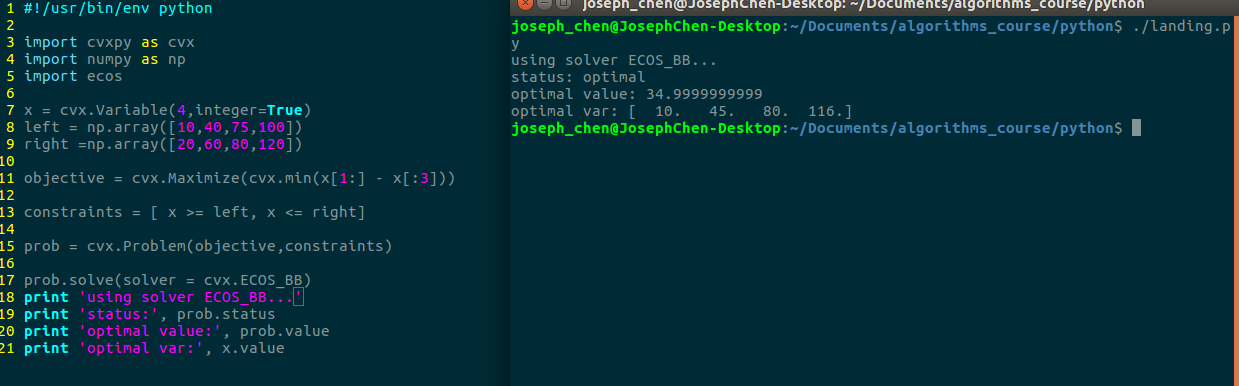
\includegraphics[width=.8\textwidth]{work4/landing}
 \end{figure}
	
\section{Palindrome Partition}
\begin{itemize}
	\item \textbf{Def.}\qquad$OPT(s,i,j)$ = the minimum cuts need for a palindrome partitioning of string $s[i \cdots j]$
	\item \textbf{Given.}\quad a string $S_n =\{s_1s_2\cdots s_n\}$
	\item \textbf{Goal.} \quad$OPT(S_n, 1, n)$  
\end{itemize}
there are several conditions , 
\begin{itemize}
	\item if $i = j$ then $OPT(s,i,j) = 0$
	\item if $s[i\cdots j]$ is a palindrome, then $OPT(s,i,j) = 0$
	\item if none of the above conditions is true, then
	\[
		OPT(s, i, j) = \min\{	
			OPT(s, i, k) + 1 + OPT(s, k+1, j)
		\}	, k = i, \cdots, j-1
	\]
\end{itemize}

We first determine whether $s_L[i\cdots j]$ is a palindrome, here $s_L$ stands for the substrings $s_L$ ($L$ from $2$ to $n$) .
\begin{algorithm}[H]
	\caption{find the minimum cuts need for palindrome partitioning }
	\begin{algorithmic}[1]
		\Require A string $S = \{s_1s_2\cdots s_n\}$
		\Ensure the minimum cuts need for $S$ 
		 \Function{mini-partition}{$S = \{s_1s_2\cdots s_n\}$}
			\State set each elements of $C[n]$ with $0$, 
			each elements of $P[n][n]$ with $True$  
			\For{$L$ from $2$ to $n$}
				\For { $i$ from $1$ to $n - L +1$ }
					\State $j = i + L- 1$
					\If {$s[i] = s[j]$ and $L = 2$}
						\State $P[i][j] = True$
					\ElsIf {$s[i] = s[j]$ and $L > 2$}
						\State $P[i][j] = P[i+1]P[j-1]$
					\Else
						\State $P[i][j] = False$ 
					\EndIf 
				\EndFor 
			\EndFor 
		 \For {$k$ from $1$ to $n$}
			 \If {$P[1][k] = True$ }
				 \State $C[k] = 0$
			 \Else
				 \State $C[k] = inf$
				 \For{$l$ from $1$ to $k-1$ }
					 \If{$P[l+1][k] = True$ and $C[k] > 1 + C[l]$}
						  \State $C[k] = 1 + C[l]$
					 \EndIf 
				 \EndFor 
			 \EndIf 
		 \EndFor 
		 \State \Return $C[n]$
		 \EndFunction 
	\end{algorithmic}	
\end{algorithm} 
\textbf{time complexity:} 
$O(n^2)$
 
	
	
\end{document}